\documentclass[a4paper]{report}
\usepackage{graphicx}
\usepackage{xcolor}
\usepackage{colortbl}
\usepackage{float}
\usepackage{soul}
\usepackage{Sweave}
\usepackage{lscape}
\usepackage{microtype}
\usepackage{hyperref}
\usepackage[section]{placeins}
\usepackage{pslatex}
\usepackage{palatino}
\usepackage{avant}
\usepackage{verbatim}
%% layout commands may be written here
%% \newcounter{}
\begin{document}
\Sconcordance{concordance:sexpr.tex:sexpr.Rnw:%
1 40 1 1 2 1 0 3 1 22 0 2 2 1 0 1 1 17 0 1 2 5 1 1 2 1 0 1 1 4 0 1 2 25 %
1 1 2 1 0 1 1 6 0 1 2 8 1 1 2 6 0 1 1 3 0 1 2 2 1 1 8 7 0 2 1 6 0 1 2 %
20 1 1 2 25 0 1 2 1 1}


\pagenumbering{arabic}



\title{Reproducible Reports with R , TEX , \& Sweave}
\author{Ivan C. Hanigan}
\date{\today}
\maketitle
\tableofcontents

\section{Introduction}
I support the philosophy of Reproducible Research \url{http://www.sciencemag.org/content/334/6060/1226.full}, and where possible I provide data and code in the statistical software R that will allow analyses to be reproduced.  This document is prepared automatically from the associated Sweave (RNW) file.  If you do not have access to the RNW file please contact me.

This is a brief intro and template to Reproducible Reports with R , TEX , \& Sweave. For a great overview of why you might want to do this see: 
Scott, T. A. (n.d.). Reproducible Research with R , TEX , \& Sweave: A common ( flawed ) approach for generating statistical reports. Retrieved from \url{http://biostat.mc.vanderbilt.edu/wiki/Main/SweaveLatex}

The basic idea is to write the narrative of your report as well as the R code to compute the results \textbf{at the same time}.  This is done within a special LaTeX file called a Sweave document.  


Sweave commands are placed inside the $\ll$ $\gg=$. Use echo to hide or show the actual R code. For figures use fig=TRUE,echo=FALSE,png=TRUE,pdf=FALSE,eps=FALSE to get the figure saved out as a separate png file instead of the default and not very useful pdf format. For tables make sure that you have the Xtable package installed in R and use echo=FALSE,results=tex.
\subsection{Some Code}
\begin{Schunk}
\begin{Sinput}
> x<-rnorm(100,10,5)
> y<-rnorm(100,20,15)
> fit <- lm(y~x)
> summary(fit)
\end{Sinput}
\begin{Soutput}
Call:
lm(formula = y ~ x)

Residuals:
    Min      1Q  Median      3Q     Max 
-37.918  -9.971   0.425   8.640  50.156 

Coefficients:
             Estimate Std. Error t value Pr(>|t|)    
(Intercept) 19.254539   3.720906   5.175 1.21e-06 ***
x            0.008045   0.326438   0.025     0.98    
---
Signif. codes:  0 ‘***’ 0.001 ‘**’ 0.01 ‘*’ 0.05 ‘.’ 0.1 ‘ ’ 1

Residual standard error: 15.02 on 98 degrees of freedom
Multiple R-squared:  6.198e-06,	Adjusted R-squared:  -0.0102 
F-statistic: 0.0006074 on 1 and 98 DF,  p-value: 0.9804
\end{Soutput}
\end{Schunk}
Using the xtable package allows results to be displyed in tables and has built in support for some R objects, so summrising the linear fit above in ~\ref{ATable}
\begin{Schunk}
\begin{Sinput}
> library(xtable)
> xtable(fit, caption="Example Table",digits=4,table.placement="H",label="ATable")
\end{Sinput}
% latex table generated in R 3.0.2 by xtable 1.7-1 package
% Wed Feb 12 14:05:07 2014
\begin{table}[ht]
\centering
\begin{tabular}{rrrrr}
  \hline
 & Estimate & Std. Error & t value & Pr($>$$|$t$|$) \\ 
  \hline
(Intercept) & 19.2545 & 3.7209 & 5.1747 & 0.0000 \\ 
  x & 0.0080 & 0.3264 & 0.0246 & 0.9804 \\ 
   \hline
\end{tabular}
\caption{Example Table} 
\label{ATable}
\end{table}\end{Schunk}
\subsection{A Plot}
 
Plots intergrate easily, using the \LaTeX float package as can be seen in figure ~\ref{test}
\begin{figure}[H]
\begin{center}
%Chunk 2
\begin{Schunk}
\begin{Sinput}
> plot(x,y,main="Example Plot",xlab="X Variable",ylab="Y Variable")
> abline(fit,col="Red")
\end{Sinput}
\end{Schunk}
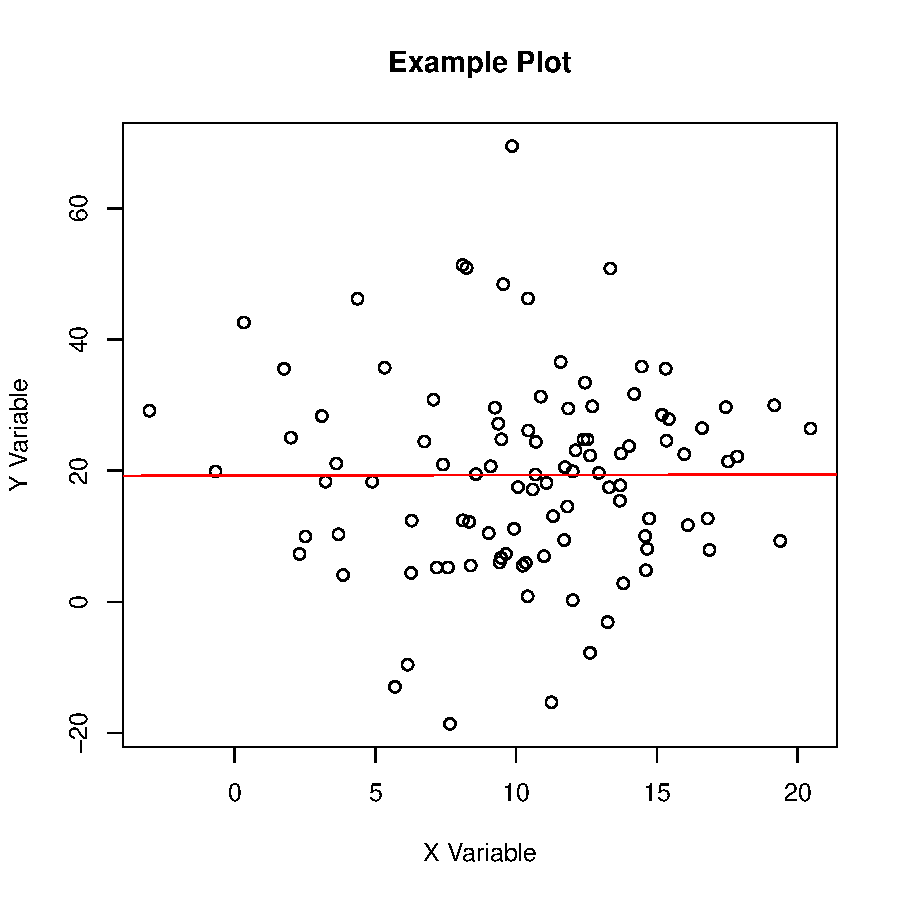
\includegraphics{sexpr-003}
\end{center}
\caption{Some Plot}
\label{test}
\end{figure}
\clearpage




\section{Inline R output}
Say we want to calculate a number and report it we can use this code:

\begin{verbatim}
One and One is \\ Sexpr{1 + 1}.
\end{verbatim}
Which will look like this: One and One is 2.

We might want to write multiple lines of R code:
\begin{verbatim}
Lm returns \\ Sexpr{x <- rnorm(100,1,1);y <- rnorm(100,0,1);summary(lm(y ~ x))$coeff[1,1];}.
\end{verbatim}

Which will look like this: Lm returns 0.0327560198919872.

\section{Inline R output with functions}
Including Functions can be tricky:
\begin{Schunk}
\begin{Sinput}
> sayhi <- function(k=2) {for(i in 1:k) cat("hi",i,"| ") }
> sayhi()
\end{Sinput}
\begin{Soutput}
hi 1 | hi 2 | 
\end{Soutput}
\end{Schunk}

But with 
\begin{verbatim}
Sexpr, {\tt sayhi()} prints <>.
\end{verbatim}

Says: Sexpr, {\tt sayhi()} prints <>.
Note that {\tt sayhi()} returns nothing; that's why Sexpr doesn't work.  But in a code chunk it does:

\begin{Schunk}
\begin{Sinput}
> a <- sayhi()
\end{Sinput}
\begin{Soutput}
hi 1 | hi 2 | 
\end{Soutput}
\begin{Sinput}
> cat(a)
\end{Sinput}
\end{Schunk}

If we rewrite the function to return the result:

\begin{Schunk}
\begin{Sinput}
> savehi <- function(k=2) {
+   out <- c()
+   for(i in 1:k) {
+     out <- paste(out, "hi", i,"| ")
+   }
+   out
+ }
> hi <- savehi()
> cat(hi)
\end{Sinput}
\begin{Soutput}
 hi 1 |  hi 2 | 
\end{Soutput}
\end{Schunk}

And with Sexpr, {\tt savehi()} prints < hi 1 |  hi 2 | >.



\section{Notes}
For the header with palatino see 
\url{http://cran.r-project.org/web/packages/lazyWeave/lazyWeave.pdf}

For eg:
\begin{verbatim}
install.packages("lazyWeave")
require(lazyWeave)
lazy.file.start(docClass="report", 
packages=c("pslatex", "palatino", "avant"), 
title="Report Name", author="Your Name")
\end{verbatim}

For the intro to including R calculations in the paragraphs (ie using 'Sexpr') see:
\url{http://tex.stackexchange.com/a/22392}.
\section{sessionInfo}
\begin{Schunk}
\begin{Sinput}
> sessionInfo()
\end{Sinput}
\begin{Soutput}
R version 3.0.2 (2013-09-25)
Platform: x86_64-redhat-linux-gnu (64-bit)

locale:
 [1] LC_CTYPE=en_US.UTF-8       LC_NUMERIC=C              
 [3] LC_TIME=en_US.UTF-8        LC_COLLATE=en_US.UTF-8    
 [5] LC_MONETARY=en_US.UTF-8    LC_MESSAGES=en_US.UTF-8   
 [7] LC_PAPER=en_US.UTF-8       LC_NAME=C                 
 [9] LC_ADDRESS=C               LC_TELEPHONE=C            
[11] LC_MEASUREMENT=en_US.UTF-8 LC_IDENTIFICATION=C       

attached base packages:
[1] stats     graphics  grDevices utils     datasets  methods   base     

other attached packages:
[1] xtable_1.7-1

loaded via a namespace (and not attached):
[1] tools_3.0.2
\end{Soutput}
\end{Schunk}

\end{document}
